\begin{frame}
  \frametitle{Hybrid $S_N$-Diffusion Method: Theory}
  \textbf{Hybrid $\bm{S_N}$-Diffusion Method}
%  \begin{block}{\textbf{Aim}}
%    To enable accurate control rod modeling in time-dependent molten salt reactor simulations
%  \end{block}
  \begin{block}{\textbf{Method Overview}}
    \begin{itemize}
      \item Applies the discrete ordinates ($S_N$) method to a small subregion around a
        control rod to generate corrections for the neutron diffusion equation
      \item Limits computationally expensive $S_N$ calculations to small subdomains
      \item Retains the computational efficiency of the neutron diffusion method
      \item Applies an adaptive algorithm to smooth flux gradients near the $S_N$-diffusion interface
    \end{itemize}
  \end{block}
  \begin{figure}
    \centering
    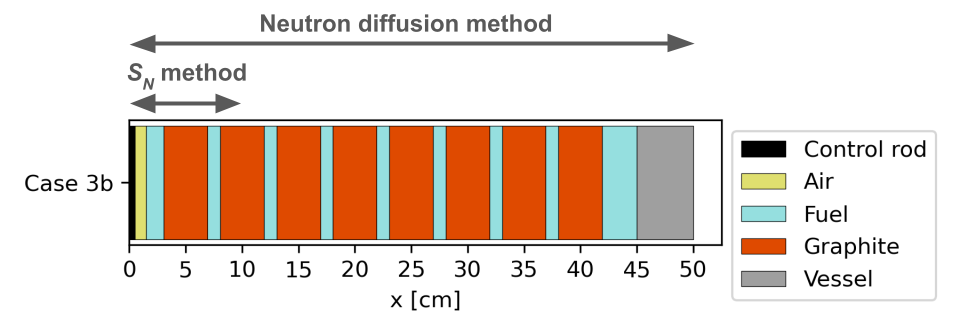
\includegraphics[width=.7\textwidth]{hybrid-illustration}
    \caption{Illustration of the problem domains of the $S_N$ and neutron diffusion methods in an
    example 1-D problem.}
  \end{figure}
\end{frame}

\begin{frame}
  \frametitle{Hybrid $S_N$-Diffusion Method: Theory}
  \textbf{Multigroup Discrete Ordinates $\bm{S_N}$ Neutron Transport Equations}
  \vspace{.2cm}

  The multigroup $S_N$ equations defined on the 3-D spatial domain 
  $\mathcal{D}$ and 2-D unit sphere angular domain $\mathcal{S}$ is:
  \begin{multline}
    \hat{\Omega}\cdot\nabla\Psi_g(\vec{r},\hat{\Omega},t) + \Sigma_{t,g}
    \Psi_g(\vec{r},\hat{\Omega},t) =
    \sum^G_{g'=1}\int_\mathcal{S} \Sigma_s^{g'\rightarrow g}(\hat{\Omega}'\rightarrow\hat{\Omega})
    \Psi_{g'}(\vec{r},\hat{\Omega}',t)d\hat{\Omega}' \\
    + \frac{1}{4\pi}\frac{\chi_{p,g}(1-\beta)}{k}\sum^G_{g'=1} \nu\Sigma_{f,g'} \phi_{g'}(\vec{r},t)
    + \frac{1}{4\pi}\sum^I_{i=1}\chi_{d,g}
    \lambda_i C_i(\vec{r},t)
    \label{eq:mg-nte}
  \end{multline}
  with boundary conditions:
  %
  \begin{gather}
    \Psi_g(\vec{r},\hat{\Omega}) = \Psi^\text{inc}_g(\vec{r},\hat{\Omega}) +
    \alpha^s_g\Psi_g(\vec{r},\hat{\Omega}_r)
    \mbox{ on } \vec{r} \in \partial\mathcal{D} \mbox{ and } \hat{\Omega}\cdot\hat{n}_b < 0,
    \shortintertext{where}
    \begin{align*}
%      \chi_{p,g} &= \mbox{prompt fission neutron spectrum in group $g$,} \\
%      \beta &= \sum^I_{i=1} \beta_i = \mbox{total delayed neutron fraction,} \\
%      \chi_{d,g} &= \mbox{delayed fission neutron spectrum in group $g$,} \\
%      \lambda_i &= \mbox{decay constant of precursor group $i$,} \\
%      C_i &= \mbox{delayed neutron precursor concentration for group $i$,} \\
      \Psi^\text{inc}_g &= \mbox{incident surface source in group $g$,} \\
      \alpha^s_g &= \mbox{specular reflectivity on }\partial \mathcal{D} \mbox{ for group }g, \\
      \hat{\Omega}_r &= \hat{\Omega}-2(\hat{\Omega}\cdot \hat{n}_b)\hat{n}_b = \mbox{reflection angle}, \\
      \hat{n}_b &= \mbox{outward unit normal vector on the boundary.}
    \end{align*}
  \end{gather}
\end{frame}

\begin{frame}
  \frametitle{Hybrid $S_N$-Diffusion Method: Theory}
  \textbf{Self-Adjoint Angular Flux (SAAF) Formulation of the Multigroup $\bm{S_N}$ Equations}
  \vspace{.2cm}

  Second-order linear neutron transport equation derived by obtaining the analytical solution of
  angular flux and substituting it back into the $S_N$ equations.

  \begin{block}{\textbf{Implementation Details}}
    \begin{itemize}
      \item Implemented with finite element method (FEM)
      \item Compatible with the efficient and scalable Hypre-BoomerAMG preconditioning
      \item Uses a modified formulation to handle $1/\Sigma_{t,g}$ factor in void regions (similar to
        Streamline-Upwind/Petrov Galerkin (SUPG) stabilization scheme) \cite{wang_diffusion_2014}
      \item Level-symmetric quadrature set for angular discretization (up to $S_{18}$)
      \item Nonlinear diffusion acceleration scheme \cite{wang_diffusion_2014}
    \end{itemize}
  \end{block}
\end{frame}

\begin{frame}
  \frametitle{Hybrid $S_N$-Diffusion Method: Theory}
  \textbf{Weak Formulation of the Multigroup SAAF $S_N$ Equations}
  \begin{gather}
    \shortintertext{Streaming term:}
    \sum^G_{g=1}\sum^{N_d}_{d=1}w_d\left(\hat{\Omega}_d\cdot\nabla\Psi^*_{g,d},\tau_g\hat{\Omega}
    \cdot\nabla\Psi_{g,d}-(1-\tau_g\Sigma_{t,g})\Psi_{g,d}\right)_\mathcal{D} \\
    \shortintertext{Collision term: }
    \sum^G_{g=1}\sum^{N_d}_{d=1}w_d\left(\Psi^*_{g,d},\Sigma_{t,g}\Psi_{g,d}\right)_\mathcal{D} \\
    \shortintertext{Scattering term:}
    \sum^G_{g=1}\sum^{N_d}_{d=1}w_d\left(\Psi^*_{g,d}+\tau_g\hat{\Omega}_d\cdot\nabla\Psi^*_{g,d},
    \sum^G_{g'=1}\sum^L_{l=0}\Sigma^{g'\rightarrow g}_{s,l}\sum^l_{m=-l}
    \frac{2l+1}{w}Y_{l,m}(\hat{\Omega}_d)\phi_{g',l,m}\right)_\mathcal{D} \\
    \shortintertext{Fission source term: }
    \sum^G_{g=1}\sum^{N_d}_{d=1}w_d\left(\Psi^*_{g,d}+\tau_g\hat{\Omega}_d\cdot\nabla\Psi^*_{g,d},
    \frac{1}{w}\frac{\chi_{p,g}(1-\beta)}{k}\sum^G_{g'=1}\nu\Sigma_{f,g'}\phi_{g'}\right)_\mathcal{D}
  \end{gather}
\end{frame}

\begin{frame}
  \frametitle{Hybrid $S_N$-Diffusion Method: Theory}
  \textbf{Weak Formulation of the Multigroup SAAF $S_N$ Equations}
  \begin{gather}
    \shortintertext{Delayed neutron source term:}
    \sum^G_{g=1}\sum^{N_d}_{d=1}w_d\left(\Psi^*_{g,d}+\tau_g\hat{\Omega}_d\cdot\nabla\Psi^*_{g,d},
    \frac{1}{w}\sum ^I_{i=1}\chi_{d,g}\lambda_i C_i\right)_\mathcal{D}
    \shortintertext{Boundary source term:}
    \begin{cases}
      \sum^G_{g=1}\sum^{N_d}_{d=1}w_d\left(\Psi^*_{g,d},
      \hat{\Omega}_d\cdot\hat{n}_b\Psi_{g,d}\right)_{\partial\mathcal{D}},
      & \hat{\Omega}\cdot\hat{n}_b>0,\vec{r}\in\partial\mathcal{D} \\
      \sum^G_{g=1}\sum^{N_d}_{d=1}w_d\left(\Psi^*_{g,d},
      \hat{\Omega}_d\cdot\hat{n}_b\Psi^\text{inc}_{g,d}\right)_{\partial\mathcal{D}},
      & \hat{\Omega}\cdot\hat{n}_b<0,\vec{r}\in\partial\mathcal{D}
    \end{cases} \label{eq:boundary-source} \\
    \shortintertext{Reflecting boundary term:}
    \begin{cases}
      \sum^G_{g=1}\sum^{N_d}_{d=1}w_d\left(\Psi^*_{g,d},
      \hat{\Omega}_d\cdot\hat{n}_b\Psi_{g,d}\right)_{\partial\mathcal{D}},
      & \hat{\Omega}\cdot\hat{n}_b>0,\vec{r}\in\partial\mathcal{D}_s \\
      \sum^G_{g=1}\sum^{N_d}_{d=1}w_d\left(\Psi^*_{g,d},
      \hat{\Omega}_d\cdot\hat{n}_b\Psi_{g,d_r}\right)_{\partial\mathcal{D}},
      & \hat{\Omega}\cdot\hat{n}_b<0,\vec{r}\in\partial\mathcal{D}_s
    \end{cases} \label{eq:reflecting-bc}
  \end{gather}
\end{frame}

\begin{frame}
  \frametitle{Hybrid $S_N$-Diffusion Method: Theory}
  \textbf{Weak Formulation of the Multigroup SAAF $S_N$ Equations}
  \begin{gather}
    \shortintertext{Void stabilization parameter \cite{wang_diffusion_2014}:}
    \tau_g =
    \begin{cases}
      \frac{1}{c\Sigma_{t,g}} \mbox{ for } ch\Sigma_{t,g} \geq \varsigma \\
      \frac{h}{\varsigma} \mbox{ for } ch\Sigma_{t,g} < \varsigma
    \end{cases}, \\
    \shortintertext{where}
    \begin{align*}
      h &= \mbox{mesh element size,} & \\
      c &= \mbox{maximum stabilization factor,} & \\
      \varsigma &= \mbox{void constant.} &
    \end{align*}
  \end{gather}
  $c=1$ and $\varsigma=0.5$ by default.
  \vspace{.2cm}

  The SAAF-$S_N$ equations require this stabilization scheme
  in near-void regions where $\Sigma_{t,g}$ is very small.
\end{frame}

\begin{frame}
  \frametitle{Hybrid $S_N$-Diffusion Method: Theory}
  \textbf{Multigroup Neutron Diffusion Equations}
  \begin{gather}
    - \nabla \cdot D_g \nabla \phi_g + \Sigma^r_g \phi_g =
    \sum^G_{g' \neq g} \Sigma^s_{g' \rightarrow g} \phi_{g'}
    + \frac{\chi_{p,g} \left( 1-\beta \right)}{k} \sum^G_{g'=1} \nu \Sigma^f_{g'}
    \phi_{g'} + \chi^d_g \sum^I_i \lambda_i C_i \label{eq:neutron} %\\
  \end{gather}
  %
  Traditionally, $D_g$ is determined through region-wide neutron interaction tallies in
  high-fidelity neutron transport simulations as follows:
  \begin{align}
    D_g =& \frac{1}{3\Sigma_{t,g}} \quad \mbox{(isotropic)} \\
    D_g =& \frac{1}{3\Sigma_{tr,g}} = \frac{1}{3\left(\Sigma_{t,g}-
    \Sigma_{s1,g}\right)}
    \quad \mbox{(linearly anisotropic)} \label{eq:p1-diffcoef}
    \shortintertext{where}
    \Sigma_{tr} =& \mbox{ macroscopic transport cross section} \nonumber
  \end{align}
\end{frame}

\begin{frame}
  \frametitle{Hybrid $S_N$-Diffusion Method: Theory}
  \textbf{Diffusion Correction Scheme (Implemented in Python)}
  \vspace{.2cm}

  In this work, I investigated two transport correction schemes. The first scheme is the diffusion
  correction scheme similar to Fick's first law of diffusion:
  \begin{gather}
    D^s_g(x) = -J^{tr}_g(x)\bigg/\frac{d\phi^{tr}_g(x)}{dx} \label{eq:svdc}
  \end{gather}
  %
  where $D^s_g$ is the diffusion correction parameter, and the $tr$ superscript denotes the
  transport-derived neutron current and scalar flux solutions from the $S_N$ method.
  \vspace{.2cm}

%  $D^s_g$ provides pointwise corrections to closely match the diffusion flux solution to the $S_N$
%  flux solution.
  By replacing $D_g$ with $D^s_g$, we are effectively adding the following transport correction term
  %
  \begin{gather}
    -\nabla\cdot (D^s_g-D_g)\nabla\phi_g
  \end{gather}
  to the neutron diffusion equations.
  \vspace{.2cm}

  $\Rightarrow$ Abandoned after 1-D investigations due to division-by-zero issues near flux maximas
  and minimas.
\end{frame}

\begin{frame}
  \frametitle{Hybrid $S_N$-Diffusion Method: Theory}
  \textbf{Drift Correction Scheme (Implemented on Moltres)}
  \vspace{.2cm}

  The second scheme is the drift correction scheme arising from adding a drift term
  ($\vec{D}_g\cdot\nabla \phi_g$) to the neutron diffusion equations:
  \begin{gather}
  \scalebox{0.95}{$
    \vec{D}_g = \frac{\sum^{N_d}_{d=1}w_d\left(\tau_g\hat{\Omega}_d\hat{\Omega}_d\cdot\nabla\Psi_{g,d}
    + \left(\tau_g\Sigma_{t,g}-1\right)\hat{\Omega}_d\Psi_{g,d}
    - \tau_g\sum^G_{g'=1}\Sigma^{g'\rightarrow g}_{s,1}\hat{\Omega}_d\Psi_{g',d}
- D_g\nabla\Psi_{g,d}\right)}{\sum^{N_d}_{d=1}w_d\Psi_{g,d}},$} \label{eq:drift} \\
  \scalebox{0.95}{$
    \gamma_g =
    \frac{\sum_{\hat{\Omega}_d\cdot\hat{n}_b > 0}w_d |\hat{\Omega}_d\cdot\hat{n}_b |
  \Psi_{g,d}}{\sum^{N_d}_{d=1}w_d\Psi_{g,d}}.$} \label{eq:bound-coef}
  \end{gather}
  \vspace{.2cm}

  The drift term also provides pointwise corrections to the neutron diffusion equations. This
  formulation is derived from the SAAF-$S_N$ equations by integrating over the angular domain and
  eliminating terms shared by the neutron diffusion equations.
\end{frame}

\begin{frame}
  \frametitle{Hybrid $S_N$-Diffusion Method: Theory}
  \textbf{$S_N$ Subsolver Boundary Conditions}
  \vspace{.2cm}

  For the hybrid $S_N$-diffusion method to converge, it requires appropriate boundary conditions for
  the $S_N$ subproblem.
  We may obtain
  the best estimate by applying the $P_1$ approximation for evaluating the neutron angular flux along
  the discrete ordinates $\hat{\Omega}_d$ of the $S_N$ angular quadrature set as follows:
  \begin{align}
    \Psi_{g,d} &\approx \frac{1}{4\pi}\left(\phi^\text{diff}_g+3\hat{\Omega}_d\cdot
    \vec{J}^\text{diff}_g\right) \nonumber \\
    &=\frac{1}{4\pi}\left(\phi^\text{diff}_g-3\hat{\Omega}_d\cdot D_g\nabla\phi^\text{diff}_g\right)
  \end{align}
  Therefore, the boundary source term for the $S_N$ subsolver is:
  \begin{gather}
    \Psi^\text{inc}_{g,d} = \frac{1}{w}
    \left(\phi^\text{diff}_g-3\hat{\Omega}_d\cdot D_g\nabla\phi^\text{diff}_g\right)
  \end{gather}
  where $w$ is the sum of weights of the level-symmetric quadrature set.
\end{frame}

\begin{frame}
  \frametitle{Hybrid $S_N$-Diffusion Method: Theory}
  \begin{columns}
    \column{.35\textwidth}
    \textbf{Hybrid $S_N$-Diffusion Method Algorithm}
    \vspace{.5cm}

  {\small
  $V_0$: Full problem domain
  \vspace{.1cm}

  $V_1$: Problem subdomain containing control rod region
  \vspace{.1cm}

  $D^{s,(i)}_g$: diffusion correction parameter in the $i$-th iteration
  \vspace{.1cm}

  $\vec{D}^{(i)}_g$: drift correction parameter in the $i$-th iteration
\vspace{4cm}}
  \column{.65\textwidth}
  \begin{figure}
    \centering
    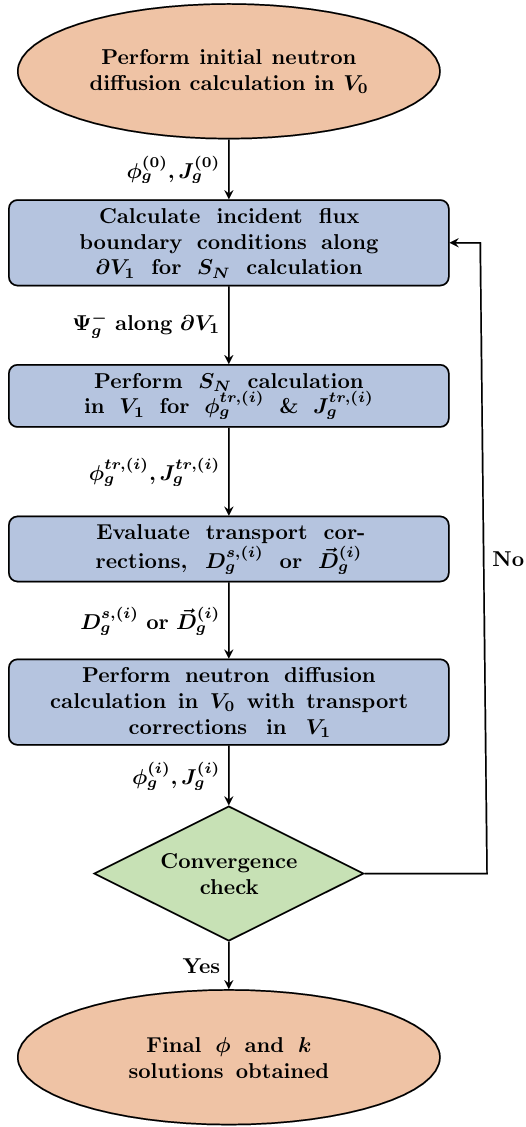
\includegraphics[width=.46\textwidth]{images/algorithm}
    \begin{minipage}[b]{.49\textwidth}
      \caption{Algorithm flowchart for the hybrid $S_N$-diffusion method.}
    \end{minipage}
  \end{figure}
\end{columns}
\end{frame}

\begin{frame}
  \frametitle{Hybrid $S_N$-Diffusion Method: Theory}
  \textbf{Correction Region ($\bm{V_1}$) and Buffer Zone}
  \begin{itemize}
    \item Recall that the full problem domain and the correction region are defined as $V_0$
      and $V_1$, where $V_1 \subseteq V_0$
    \item The approximate $S_N$ boundary conditions will generally yield some deviations in the
      flux distribution since neutron fluxes in realistic reactor systems are at least slightly
      anisotropic throughout most of the system
    \item However, the influence of boundary conditions on the ratio of $J$ and $\frac{d\phi}{dx}$
      does not extend far from the boundary $\partial V_1$ in optically thick media; transport
      correction parameters are accurate everywhere except near $\partial V_1$
    \item There exists a buffer zone near $\partial V_1$ where transport correction parameters
      are inaccurate
  \end{itemize}
%  \pause
%  $\Rightarrow$ Approach for preliminary results: Define $V_1$ such that it is large enough to
%  provide sufficient transport
%  corrections and accommodate inaccurate SVDCs near $\partial V_1$. Discard inaccurate SVDCs
%  in favor of the default $P_1$-based diffusion coefficients.
\end{frame}

\begin{frame}
  \frametitle{Hybrid $S_N$-Diffusion Method: Theory}
  \textbf{Correction Region ($\bm{V_1}$) and Buffer Zone}
  \begin{figure}[htb!]
    \centering
    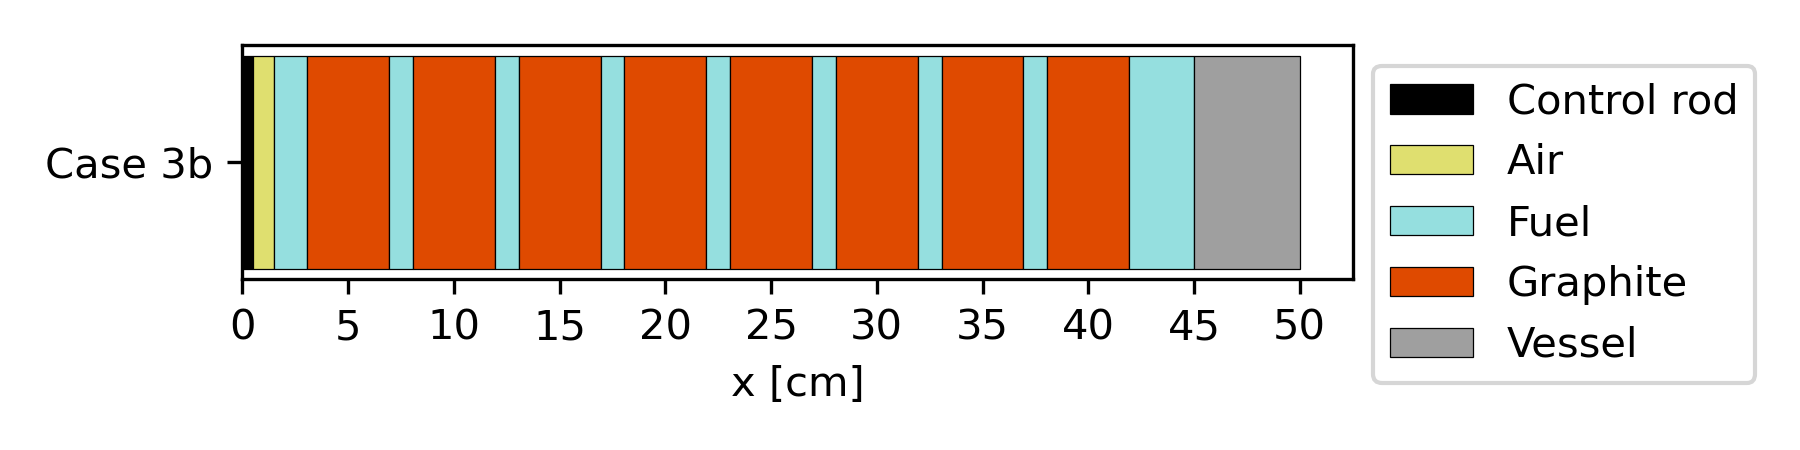
\includegraphics[width=.5\columnwidth]{case-3b-geometry}
    \caption{1-D geometry for Case 3b.}
    \label{fig:3b-geometry}
  \end{figure}
  \begin{figure}[htb!]
      \centering
      \begin{subfigure}[t]{.49\textwidth}
          \centering
          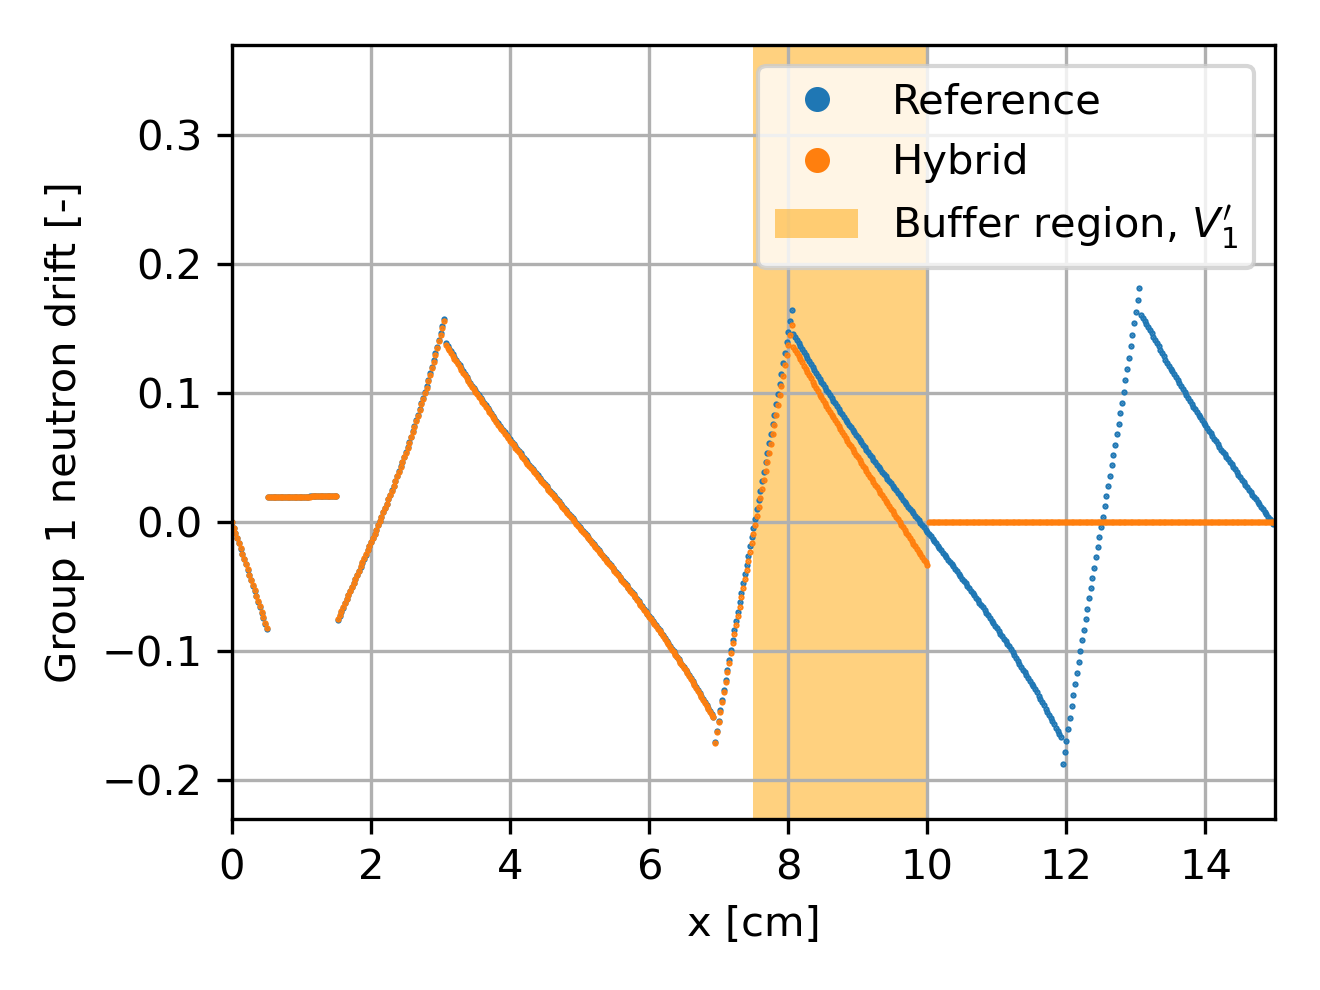
\includegraphics[width=.9\textwidth]{case-3b-group-1-drift}
      \end{subfigure}
      \hfill
      \begin{subfigure}[t]{.49\textwidth}
          \centering
          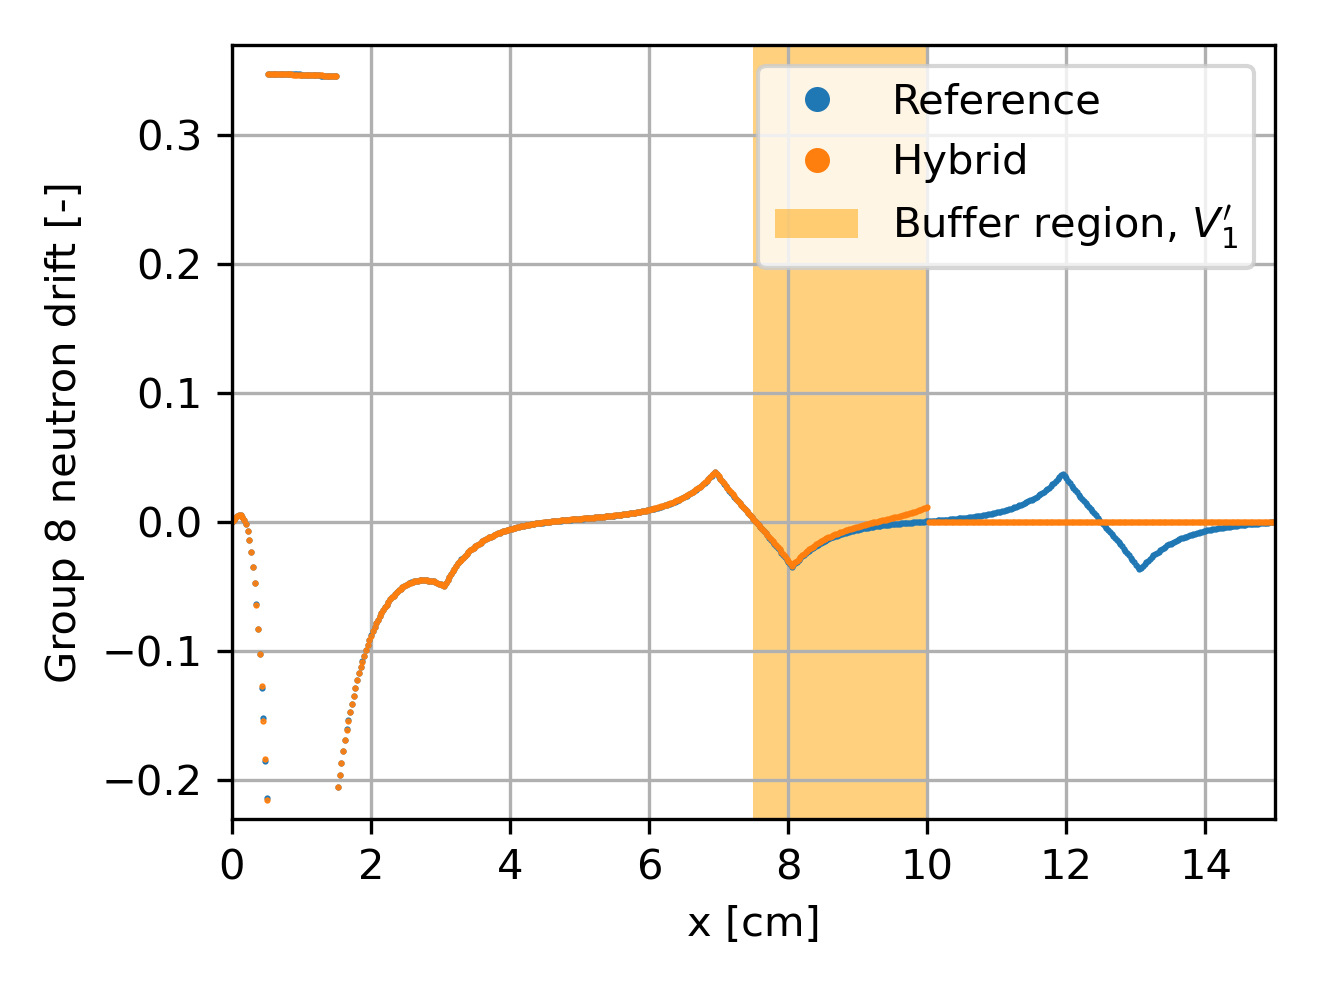
\includegraphics[width=.9\textwidth]{case-3b-group-8-drift}
      \end{subfigure}
      \caption{The reference and hybrid drift ($\vec{D}_g$) distributions for group 1 and 8 calculated
        from $S_8$ and $S_8$-diffusion simulations. The correction subregion $V_1$ spans $x=0$ cm to
        $x=10$ cm.}
      \label{fig:3b-drift-1}
  \end{figure}
\end{frame}

\begin{frame}
  \frametitle{Hybrid $S_N$-Diffusion Method: Theory}
  \textbf{Correction Region ($\bm{V_1}$) and Buffer Zone}
  \vspace{.2cm}

  A natural/intuitive criterion for the location of the buffer zone cutoff boundary
  would be wherever the components of the drift correction variable $\vec{D}_g$ is zero, i.e.,
  wherever the components change signs.
  \begin{enumerate}
    \item At points where the $\vec{D}_g$ components are zero, the flux is approximately isotropic
      along the axes corresponding to the components.
    \item This choice preserves the smoothness of the neutron flux gradient.
  \end{enumerate}
  \begin{figure}[htb!]
      \centering
      \begin{subfigure}[t]{.49\textwidth}
          \centering
          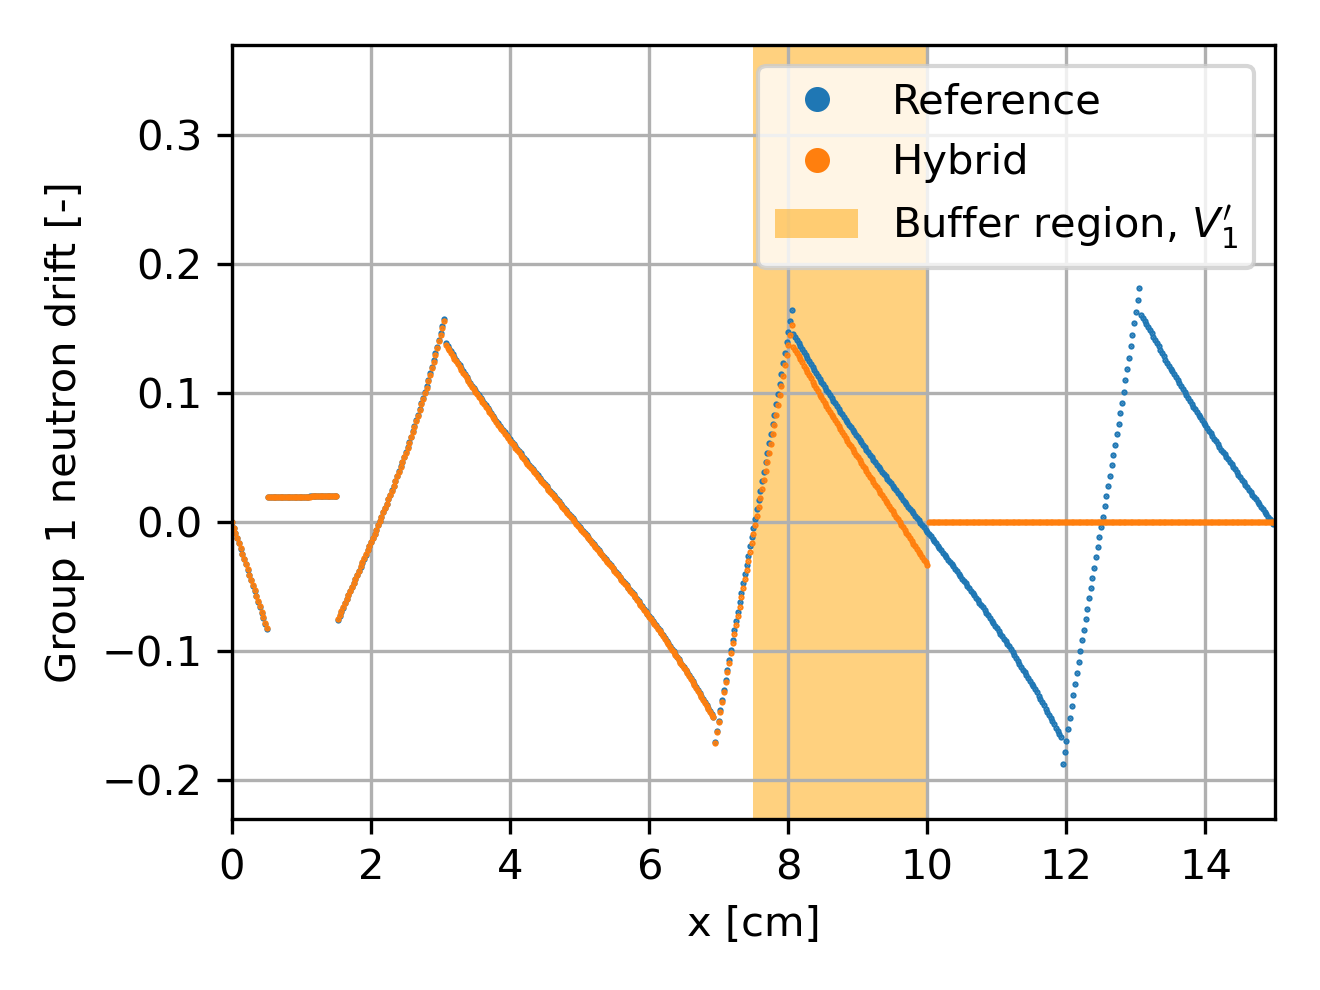
\includegraphics[width=.9\textwidth]{case-3b-group-1-drift}
      \end{subfigure}
      \hfill
      \begin{subfigure}[t]{.49\textwidth}
          \centering
          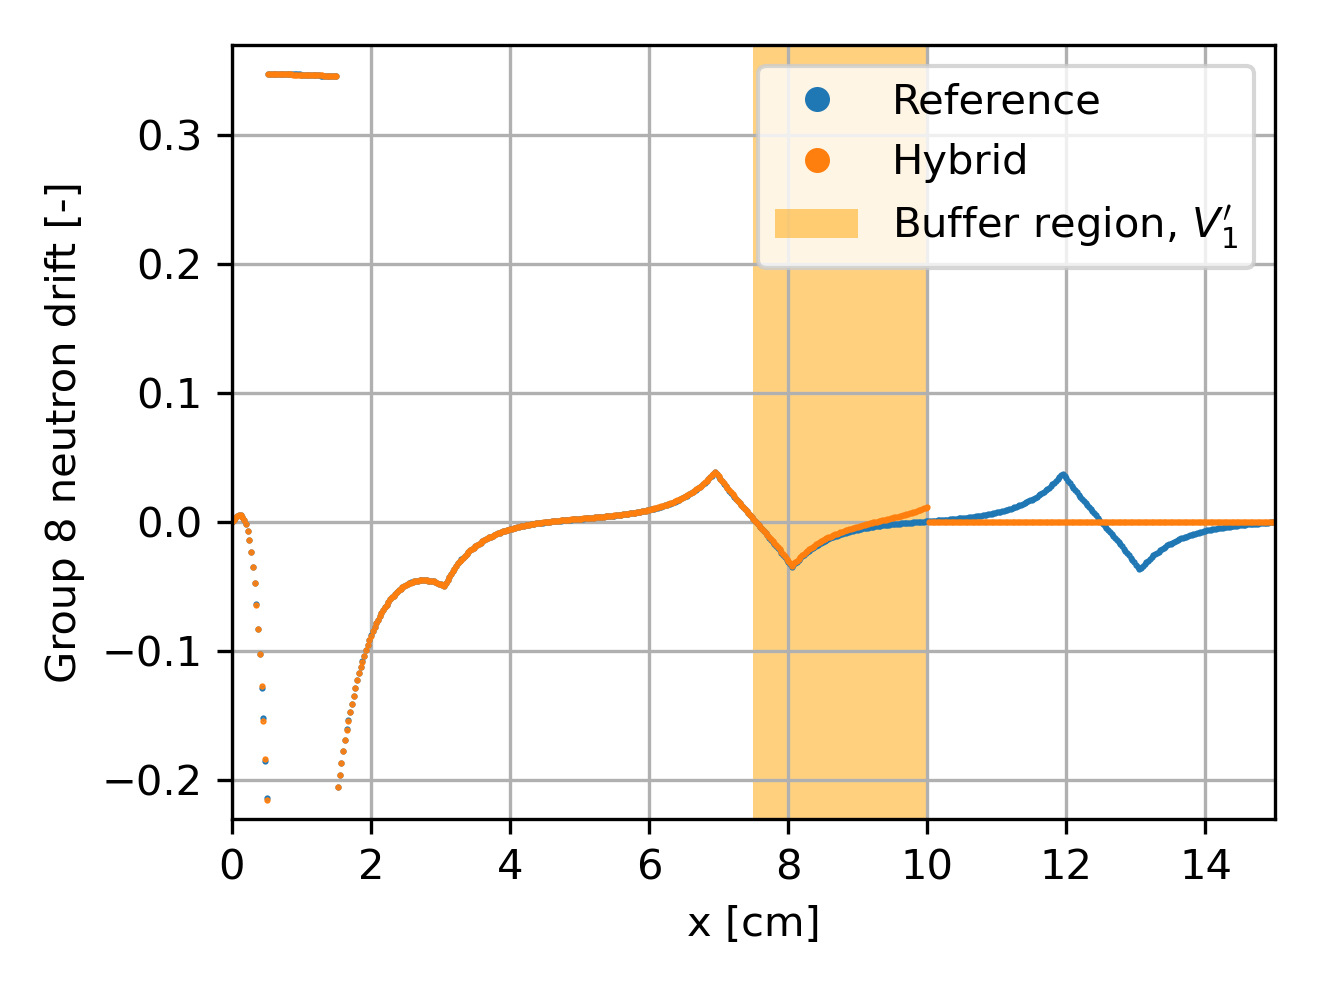
\includegraphics[width=.9\textwidth]{case-3b-group-8-drift}
      \end{subfigure}
      \caption{The reference and hybrid drift ($\vec{D}_g$) distributions for group 1 and 8 calculated
        from $S_8$ and $S_8$-diffusion simulations. The correction subregion $V_1$ spans $x=0$ cm to
        $x=10$ cm.}
      \label{fig:3b-drift-1}
  \end{figure}
\end{frame}

\begin{frame}
  \frametitle{Hybrid $S_N$-Diffusion Method: Theory}
  \textbf{Numerical Implementation}
  \vspace{.2cm}

  The SAAF-$S_N$ and hybrid $S_N$-diffusion method with the drift correction scheme were
  implemented on Moltres.
  \begin{itemize}
    \item Preconditioned Jacobian-free Newton-Krylov (PJFNK) solver \cite{knoll_jacobian-free_2004}
    \item Hypre-BoomerAMG (Algebraic multigrid) preconditioning \cite{hypre_hypre_2022}
    \item MultiApp and Transfers systems from MOOSE for iterative coupling and data transfers
    \item Supporting material and utility C++ classes for loading group constant data and performing
      angular quadrature calculations
  \end{itemize}
  \vspace{.2cm}

  A 1-D hybrid $S_N$-diffusion method with the diffusion correction
  scheme was implemented in Python. (This scheme was abandoned after 1-D analyses due to division by
  zero errors wherever the flux gradients approach zero.)
  \begin{itemize}
    \item 1-D $S_N$ method with diamond differencing scheme
    \item 1-D neutron diffusion method with finite differencing scheme
  \end{itemize}
\end{frame}
